\chapter{Architektur des Prototypen}
\label{chp:architecture}


% Warum für Framework / Technologie entschieden?
% - GraphQL wegen Graph Daten
% - Springframework wegen einfacher Entwicklung

% Mockup für API entwickeln, um parallele Programmierung des Front- und Backend zu ermöglichen (Projektmanagement)

Unser Prototyp verarbeitet die Daten von Siemens auf eine performante Art und Weise. Zuerst werden die Fehlerdaten im ausfallsicheren Messaging System Kafka von Apache geschrieben. Diese Nachrichten werden anschließend vom Backend-System, welches aus einer relationalen Datenbank (PostgreSQL) und dem Java Spring Framework besteht, verarbeitet. Außerdem stellt das Backend diese Daten mittels GraphQL-API zur Verfügung. Somit kann das Frontend, welches mit Angular implementiert worden ist, die Daten via Abfragen visualisieren.

\begin{figure}
    \centering
    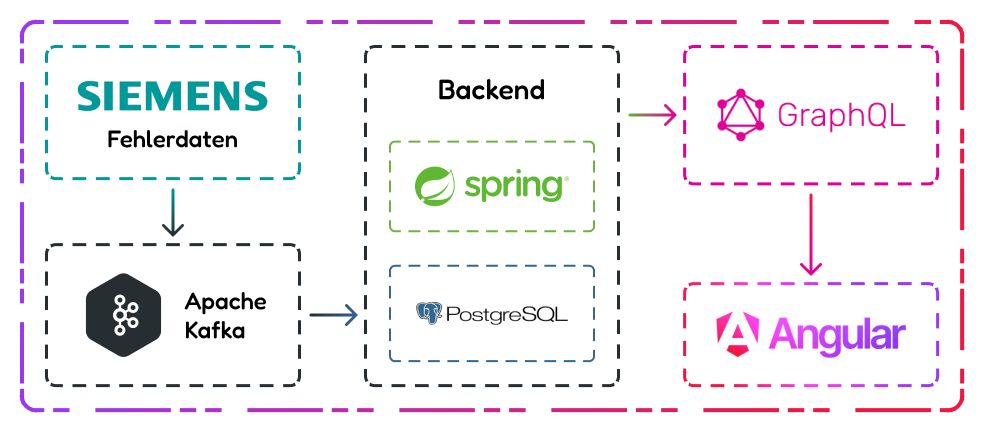
\includegraphics[width=1\textwidth]{content/img/Architecture/Architecture.jpg}
    \caption{Übersicht der Architektur unseres Prototypen}
    \label{fig:OverviewArchitektur}
\end{figure}

In diesem Kapitel werden die einzelnen Komponenten dieser Service-Oriented-Architecture (kurz SOA) im Detail beschrieben und erläutert.

\section{Apache Kafka und das Backend}
\label{chp:architecture_backend}

Die Implementierung dieses Systems basiert auf einer Architektur, die auf Apache Kafka, dem Java Spring Framework und PostgreSQL aufbaut. In diesem Kapitel wird der Ablauf der Datenverarbeitung von der Fehleranalyse bis zur Bereitstellung der Daten durch die GraphQL-API beschrieben. Ergänzend dazu werden die verwendeten Technologien im Detail erläutert und die Gründe für ihre Auswahl dargelegt.

\subsection{Messaging Service: Apache Kafka}

Die Daten werden zunächst durch die Siemens GNA Software, die für die Fehleranalyse zuständig ist, erfasst. Diese Daten werden kontinuierlich an ein Apache Kafka-Cluster gesendet, wie in der Abbildung \ref{fig:KafkaArchitektur} erkennt werden kann. Apache Kafka fungiert dabei als zentraler Datenstrom, der die Ereignisse oder Nachrichten empfängt und speichert. Hierbei gewährleistet Kafka eine zuverlässige und skalierbare Datenübertragung. Außerdem wird durch Apache Kafka eine starke Entkopplung zwischen der Siemens GNA Software und dem Backend-System hergestellt. Das Backend profitiert vor allem von der hohen Datendurchsatzrate, welche Apache Kafka erreichen kann, denn nach jeder Auswertung der Fehler im Netzdatenmodell wird eine hohe Menge an Daten dem Backend übertragen. Die Technologie Apache Kafka ist schon genauer im Kapitel \ref{kakfaExplained} beschrieben worden. Wie Apache Kafka aufgesetzt und in das Backend integriert worden ist, wird im Kapitel \ref{apacheKafkaImpl} genauer erklärt.

\begin{figure}
    \centering
    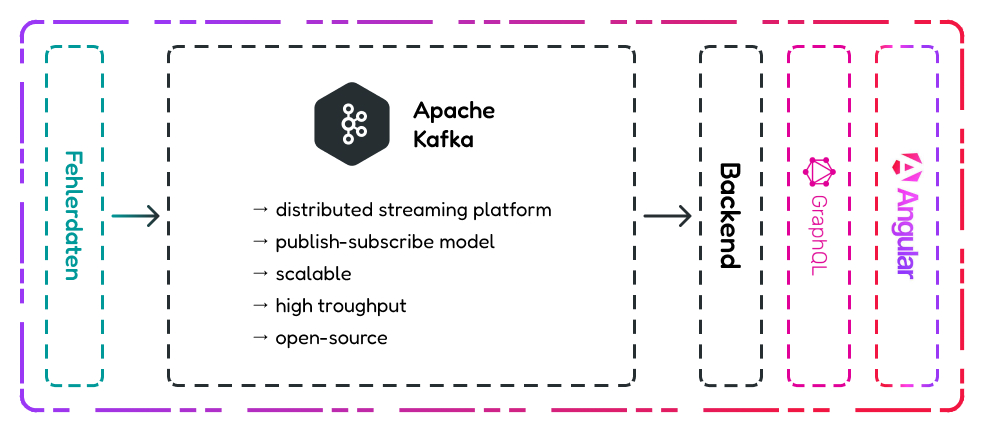
\includegraphics[width=1\textwidth]{content/img/Architecture/Architecture_Kafka.jpg}
    \caption{Architektur unseres Prototyps mit Fokus auf Kafka}
    \label{fig:KafkaArchitektur}
\end{figure}
\FloatBarrier

\subsection{Logik im Backend: Spring Framework}

Das Backend-System, das mit dem \emph{Java Spring Framework} entwickelt worden ist, ist für die Verarbeitung der empfangenen Daten zuständig, dies ist auch in der Darstellung \ref{fig:BackendArchitektur} zu sehen.  Mithilfe von \emph{Spring for Apache Kafka}, welches die Integration von Kafka in Spring ermöglicht, werden die Daten von Apache Kafka abgefragt und an das Backend weitergeleitet. In Spring werden diese Daten dann entsprechend verarbeitet und für die Speicherung in der Datenbank vorbereitet.

\begin{figure}
    \centering
    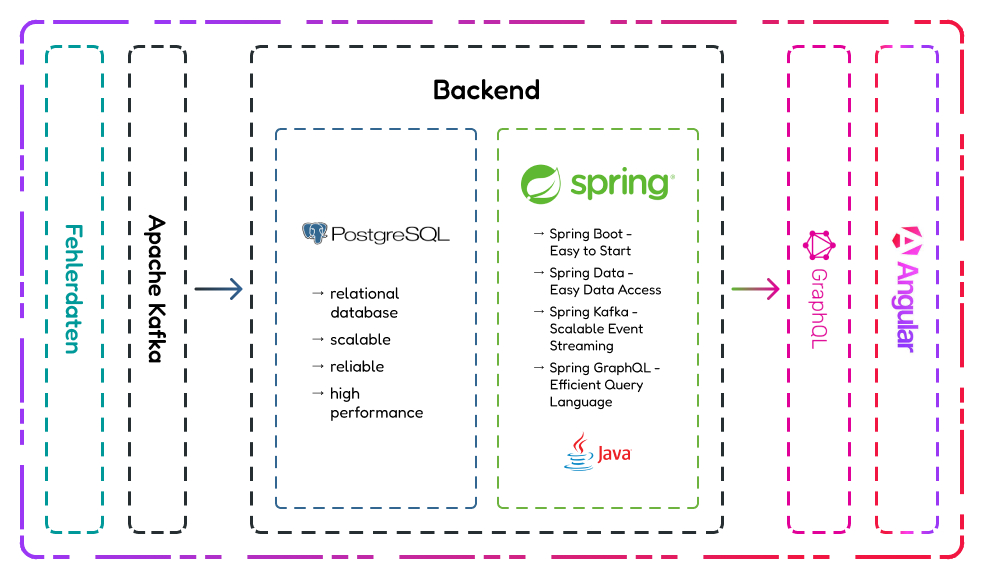
\includegraphics[width=1\textwidth]{content/img/Architecture/Architecture_Backend.jpg}
    \caption{Architektur unseres Prototyps mit Fokus auf das Backend}
    \label{fig:BackendArchitektur}
\end{figure}
\FloatBarrier

Die Entscheidung für Java als Programmiersprache und Spring als Application-Framework ist im Wesentlichen aus zwei Gründen gefällt worden. Einerseits ist die Verwendung von diesen Technologien eine fixe Anforderung seitens Siemens gewesen. Auf der anderen Seite bieten sie immense Vorteile für die Entwicklung der Anwendungen in Bezug auf unsere spezifischen Nutzungsszenarien. In den folgenden Abätzen werden diese Technologien vorgestellt und ihre Vorteile genauer beleuchtet.

Java ist eine objektorientierte, plattformunabhängige Programmiersprache, die ursprünglich von Sun Microsystems entwickelt worden ist und jetzt von Oracle Corporation gepflegt wird. Sie ist in den 1990er Jahren eingeführt worden und hat sich seitdem zu einer der beliebtesten Programmiersprachen entwickelt, insbesondere für die Entwicklung von Unternehmensanwendungen, Webanwendungen, mobilen Anwendungen und großen Systemen. \cite{javaDocs}

Ein wichtiges Konzept von Java ist die objektorientierte Programmierung (OOP). Das bedeutet, dass alles in Java als Objekt betrachtet wird. Objekte sind Instanzen von Klassen, die Daten und Methoden zur Manipulation dieser Daten enthalten. OOP-Konzepte wie Vererbung, Polymorphismus und Kapselung werden in Java stark unterstützt. Dadurch kann eine intuitive und effiziente Programmierung erreicht werden, was eine schnelle Entwicklung von Anwendungen ermöglicht. \cite{javaDocs}

Ein großer Selling-Point dieser Programmiersprache ist die Plattformunabhängigkeit. Java-Programme werden in Bytecode kompiliert, der auf der \emph{Java Virtual Machine (JVM)} ausgeführt wird. Dadurch sind Java-Anwendungen plattformunabhängig, was bedeutet, dass sie auf verschiedenen Betriebssystemen wie Windows, macOS und Linux ausgeführt werden können, solange eine JVM verfügbar ist. \cite{javaDocs}

Ein weiterer Vorteil ist die Unterstützung von \emph{Multi-Threading}, welches Anwendungen erlaubt, parallel mehrere Aufgaben abzuarbeiten. Dies ist besonders in Anwendungsfällen, welche eine große Last auf Anwendungssysteme ausüben, zum Beispiel bei Server-Systemen, von Vorteil. Außerdem hat Java ein reichhaltiges Ökosystem an Erweiterungen, wie zum Beispiel Frameworks oder Bibliotheken. Dies liegt daran, dass Java eine sehr große Popularität im Enterprise-Sektor geniest. Denn die Unternehmen, welche Java verwenden, unterstützen die Entwicklung von diesen Erweiterungen, damit ihre Produkte verlässlich und effektiv funktionieren. Aus all diesen Gründen ist die Verwendung von Java in Fall dieser Arbeit optimal. \cite{javaDocs,FireshipJava}

Das Java Spring Framework ist eine Erweiterung von Java, welche eine einfache Entwicklung von robusten, skalierbaren und wartbaren Anwendungen ermöglicht. Definitionsgemäß ist Spring ein \emph{Application-Framework} und ein \emph{Inversion of Control Container}. Ein Application-Framework ist ein strukturierter Satz von Bibliotheken, Komponenten und Tools, der die Entwicklung von Anwendungen erleichtert, indem er eine grundlegende Struktur und Funktionalität bereitstellt. Es werden komplexe Aspekte der Anwendungsentwicklung, welche grundsätzlich bei jeder Applikation gleich sind, wie der Netzwerk- oder Datenbankzugriff, abstrahiert. Damit kann der Fokus der Entwickler auf die eigentliche Anwendungslogik gelenkt werden und Ressourcen für die Erstellung von redundanten Komponenten eingespart werden. Um Probleme bei der Wiederverwendung zu vermeiden, wird auf das Konzept der Standardisierung gesetzt, welche eine zuverlässige Nutzung durch klar definierte Regeln schafft. \cite{springDocs}

Mit Inversion of Control ist eine Entwicklungstechnik gemeint, welche es ermöglicht, Objekte zu erstellen und ihre Abhängigkeiten dynamisch einzufügen. Dies fördert eine niedrige Kopplung zwischen den verschiedenen Komponenten einer Anwendung und erleichtert das Testen der Applikation. Das Java Spring Framework bietet in diesem Kontext die Umgebung an, welche das dynamische Auflösen und Einfügen von Abhängigkeiten in den Anwendungskomponenten ermöglicht. \cite{springDocs}

Der bedeutendste Vorteil in der Verwendung von Spring in Bezug auf diese Arbeit ist die leichte Integration von verschiedenen Technologien in die Anwendung durch die unzähligen Erweiterungen von diesem Framework. Beispielsweise ist die Einbindung der PostgreSQL Datenbank über die \emph{Spring Data JDBC} Bibliothek mit Leichtigkeit getätigt worden -- eine genauere Erklärung darüber ist im Kapitel \ref{postgresImpl}. Des Weiteren wird \emph{Kafka for Spring Framework} für das Interagieren des Backend-Systems mit Apache Kafka verwendet, welche auch eine Erweiterungsbibliothek ist -- eine detailreiche Erläuterung dazu ist im Kapitel \ref{apacheKafkaImpl}.

\subsection{Persistierung der Daten: PostgreSQL Datenbank}

Die verarbeiteten Daten werden in einer PostgreSQL-Datenbank persistiert. \emph{PostgreSQL} bietet eine robuste und leistungsstarke relationale Datenbanklösung, die die Anforderungen an die Datenspeicherung erfüllt. Das Java Spring Backend kommuniziert über Spring Data JDBC mit der Datenbank, um die Daten effizient zu speichern und abzurufen. Der ausschlaggebendste Grund zur Wahl von PostgreSQL ist die Anforderung von Siemens, dass eine relationale Datenbank verwendet werden soll, welche schon dem kooperierenden Entwicklungsteam von Siemens bekannt ist. Ein weiterer Grund ist die starke Popularität unter den Entwicklern und die starke Etablierung am Markt seitens PostgreSQL. In den nächsten Absätzen wird PostgreSQL und seine Vorteile genauer erklärt. 

PostgreSQL ist ein leistungsstarkes Open-Source-Datenbankmanagementsystem (DBMS), das auf dem objektrelationalen Datenbankmodell basiert. Außerdem unterstützt PostgreSQL Transaktionen, die es ermöglichen, eine Gruppe von Operationen als eine einzige atomare Einheit auszuführen. Das \emph{ACID}-Prinzip (Atomicity, Consistency, Isolation, Durability) wird unterstützt, was die Datenintegrität sicherstellt. Ein weiterer Vorteil von PostgreSQL ist, dass es in der Lage ist, als Hochverfügbarkeitsdatenbank zu operieren. Denn es können Daten zwischen mehreren Datenbankservern repliziert werden und somit kann bei einem Ausfall von einem DB-Server ein anderer die Arbeit übernehmen. 
Relationale Datenbanken haben ein sehr einfaches Konzept. Es ist aufgebaut auf Tabellen, welche Relationen zueinander haben, das heißt es können Zeilen aus verschiedenen Tabellen in Verbindung stehen, wobei jede Zeile eine Sache beschriebt. Beispielsweise könnte einer Person eine Adresse zugeordnet werden durch eine Relation zwischen einer Personentabelle und Adresstabelle. Jedoch haben relationale Datenbanken einen Haken, wenn die Daten zu stark vernetzt sind, dann kommt diese Technologie an seine Grenzen. Im Falle dieser Arbeit sind die zu verwaltende Daten Graphdaten, was stark vernetzte Daten sind, wie trotzdem eine effiziente Speicherung und performantes Abfragen gelungen ist, wird im Kapitel \ref{postgresImpl} beschrieben.  \cite{postgreSQLDocs, FireshipPostgreSQL}
\newpage
\section{GraphQL und das Frontend}
\label{chp:architecture_frontend}

Diese Sektion erklärt kurz die technische Implementierung des Frontends mit zugehörigen Services in der Architektur. Wenn Sie sich Abbildung \ref{fig:FrontendArchitektur} noch einmal ansehen, können Sie erkennen, dass die Daten über die GraphQL API vom Frontend abgerufen werden können. Dieses ist mit \emph{Angular} implementiert. Für die Visualisierung des Graphen wird die Bibliothek \emph{Cytoscape} verwendet.

\begin{figure}
    \centering
    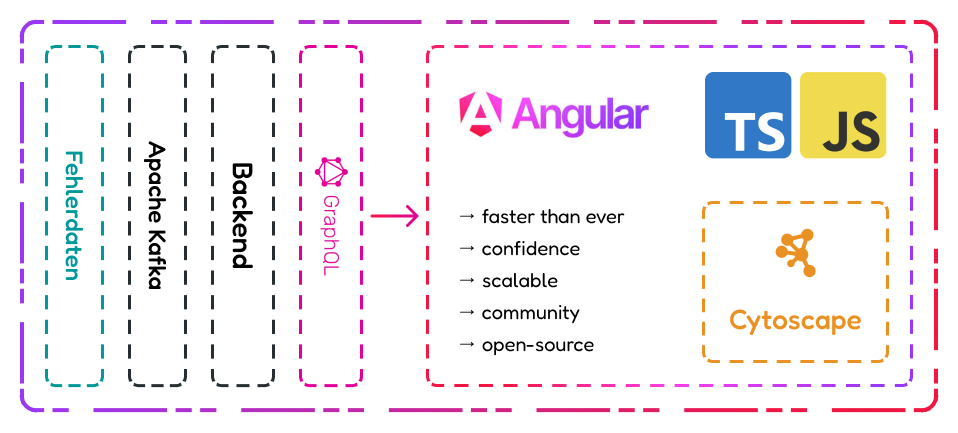
\includegraphics[width=1\textwidth]{content/img/Architecture/Architecture_Angular.jpg}
    \caption{Architektur unseres Prototypen mit Fokus auf das Frontend}
    \label{fig:FrontendArchitektur}
\end{figure}
\FloatBarrier

\subsection{Schnittstelle zwischen Backend und Frontend: GraphQL}

Eine populäre Schnittstelle für Daten, welche eine Form von Graphstruktur aufweisen, ist \emph{GraphQL}. Die Besonderheit dieser API ist die deklarative Natur der Schnittstelle. Im Gegensatz zu REST, gRPC und anderen APIs bestimmt bei GraphQL der Client, welche Eigenschaften und Felder er erhalten möchte. Dadurch wird die Transportmenge an Daten über das Internet reduziert. \cite{GraphQLWhyGraphQL}

Um im Folgenden die besonderen Eigenschaften von GraphQL näher zu erläutern, wird nun ein Beispiel eingeführt. Dabei hat ein Benutzer einen Benutzernamen und eine normalisierte Adresse. Da diese Daten aus der realen Welt am besten in einem Graphen anstatt einer Tabelle abgebildet werden können, sehen Sie in Abbildung \ref{fig:GraphExampleUserAddress} diese Abstraktion der Daten.

\begin{figure}
    \centering
    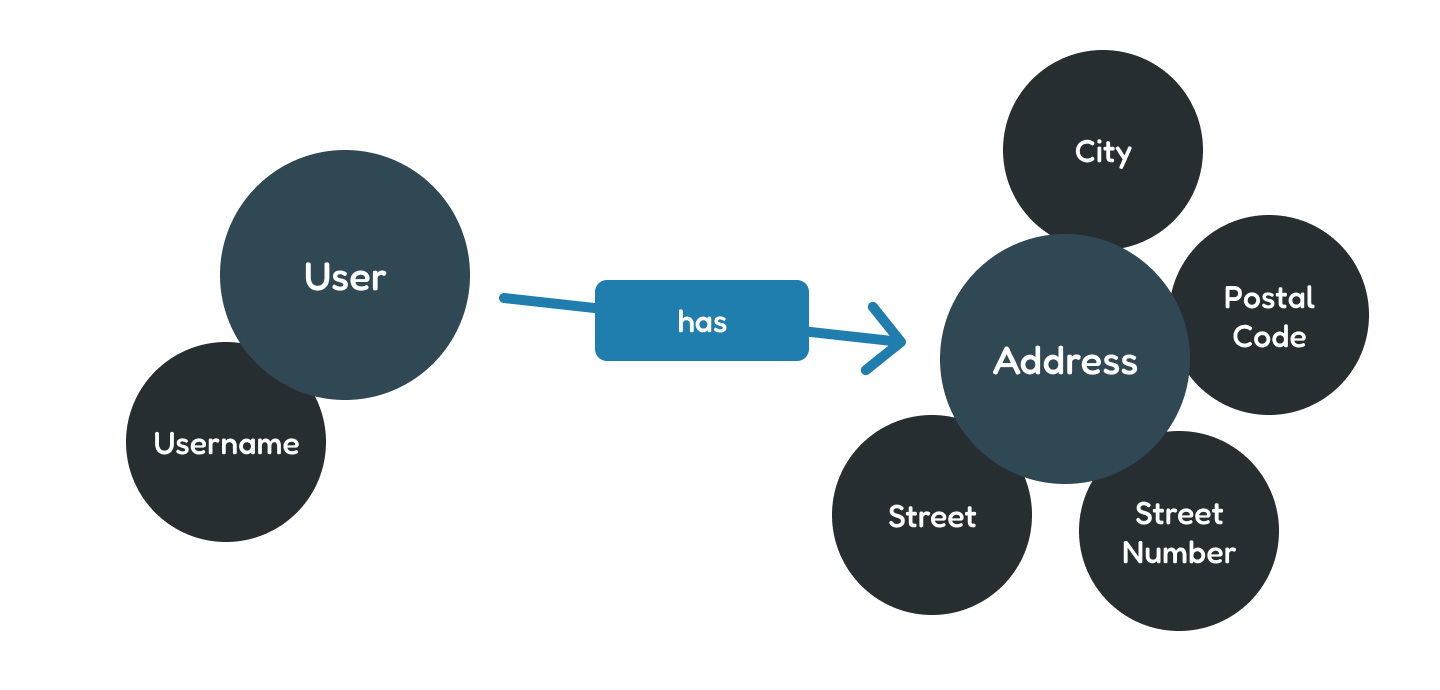
\includegraphics[width=0.8\textwidth]{content/img/Empire/Frontend/GraphQL_Example_User_Address.png}
    \caption{Speicherung von Daten unseres Beispieles in einem Graphen}
    \label{fig:GraphExampleUserAddress}
\end{figure}
\FloatBarrier

GraphQL hat den weiteren Vorteil, dass die Anzahl an Abfragen, welche durchgeführt werden müssen, um alle notwendigen Informationen zu erhalten, erheblich reduziert wird. Viele der herkömmlichen APIs benötigen eine Abfrage für die Basisinformationen (Benutzernamen) und anschließend eine weitere Abfrage für die Adresse. Dies rührt daher, weil Daten aus der realen Welt meistens eine hohe Komplexität aufweisen, und in relationalen Datenbanken in verschiedenen Tabellen gespeichert werden. GraphQL bietet Möglichkeiten, um alle Informationen, welche den Benutzer betreffen in einer Abfrage abzuhandeln. Der Client nimmt sich dann nur die Daten, die für den speziellen Use-Case gebraucht werden. \cite{FireshipGraphQL}

Außerdem wird bei GraphQL zuerst ein Schema definiert, welches laut GraphQL-Dokumentation wie eine \wordindoublequotes{Shared Language}, also geteilte Sprache, sein soll. Das gesamte Business Modell soll mittels natürlicher Sprache beschrieben werden können und genau so im Schema verwirklicht werden. Beim \wordindoublequotes{schema-first-approach} wird dieses Schema als aller erstes definiert, sodass Backend und Frontend darauf aufbauend gleichzeitig programmiert werden können. Ein kleiner Teil unseres Schemas kann im Quellcode \ref{lst:GraphQLSchema} angesehen werden. \cite{GraphQLThinkingInGraphs}

\begin{lstlisting}[language={graphql},caption={Teil unseres GraphQL Schemas},label={lst:GraphQLSchema},captionpos=b]
type ModelObject {
    guid: ID!
    name: String!
    connections: [Connection!]!
}

type Connection {
    guid: ID!,
    modelObjectGuid: ID!,
    included: Boolean!
}
\end{lstlisting}

Und genau das sind die Gründe, warum wir uns für GraphQL entschieden haben. Im Gegensatz zum Backend, wo das Java Spring Framework vorgeschrieben war, weil viele Systeme und Applikation von Siemens und auch allgemein auf der gesamten Welt mittels Java laufen und demnach die Wartbarkeit höher ist, wenn die Ingenieure keine neue Sprache erlernen müssen, hatten wir bei der API die freie Auswahl.

GraphQL basiert auf \emph{Queries} und \emph{Mutation}, wobei eine Query immer nur zum Abfragen von Daten dient und eine Mutation Daten am Server beziehungsweise in der Datenbank verändert. Die Schönheit von GraphQL liegt in der Einfachheit dieser Abfragen: \cite{GraphQLQueriesAndMutations}

\begin{lstlisting}[language={graphql},caption={Beispiel einer GraphQL-Abfrage},captionpos=b]
query {
  user (input: {id: 69}) {
    __typename
    ... on UserResult {
      username
      address {
        street
        streetNumber
      }
    }
    ... on Error {
      cause
    }
  }
}
\end{lstlisting}

Für die verschiedenen Typen dieser Abfrage sind noch weitere Felder, wie zum Beispiel die Postleitzahl oder die Stadt verfügbar. Jedoch benötigt der Client in diesem Fall dieser Werte nicht, weswegen die Daten nicht übertragen werden müssen. 

\begin{lstlisting}[language={json},caption={Rückgabe einer GraphQL-Abfrage},captionpos=b]
{
  "data": {
    "user": {
      "__typename": "UserResult",
      "result": {
        "username": "trueberryless",
        "address": {
          "street": "An Der Bundesstrasse",
          "streetNumber": 4,
        }
      }
    }
  }
}
\end{lstlisting}

Mithilfe dieser Technologie werden die Daten aus dem Backend nun zur Verfügung gestellt. Dabei unterstützt unsere API eine Menge an Schnittstellen, welche in der Abbildung \ref{fig:GraphQLQueries} eingesehen werden können. Alle diese Abfragen sind für die Implementierung des Frontends notwendig und äußerst nützlich. Dabei muss wieder bedacht werden, dass nicht unbedingterweise alle Felder der Abfrage in Verwendung treten müssen, da bei GraphQL der Client entscheidet, welche Daten er erhalten möchte. \cite{GraphQLWhyGraphQL}

\begin{figure}
    \centering
    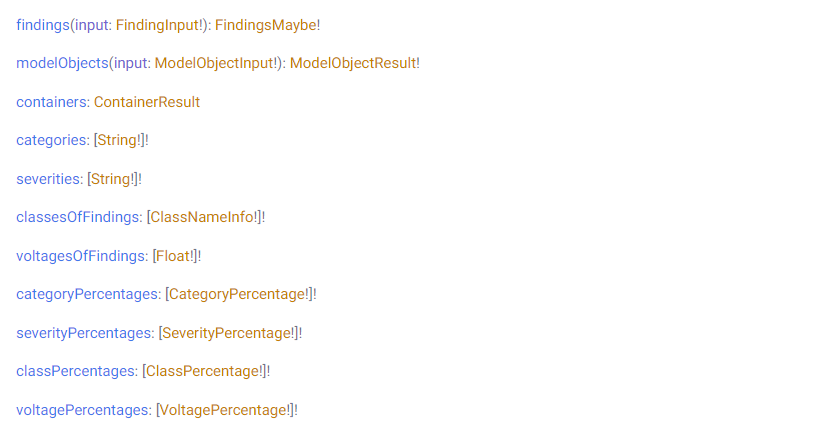
\includegraphics[width=0.8\textwidth]{content/img/Empire/Frontend/Queries.png}
    \caption{Auflistung der Abfragen, welche mittels GraphQL implementiert sind [Schema Definition]}
    \label{fig:GraphQLQueries}
\end{figure}
\FloatBarrier

\subsection{Framework aus der JavaScript Welt: Angular}

Das von Google entwickelte, auf der Programmiersprache TypeScript aufbauende Framework \emph{Angular} ist erstmals 2009 als Nebenprojekt von Misko Hevery und Adam Abrons am Markt erschienen (damals noch AngularJS) und wird aktiv seit 2016 von Google weiterentwickelt. Erst im November 2023 hat Angular ein neues Aussehen bekommen und hat ab Version 17 nun auch ein modernes Logo. Wie Angular in unser System integriert ist, sehen Sie in der Darstellung \ref{fig:ArchitectureFrontendAngular}. \cite{FireshipAngular}

\begin{figure}
    \centering
    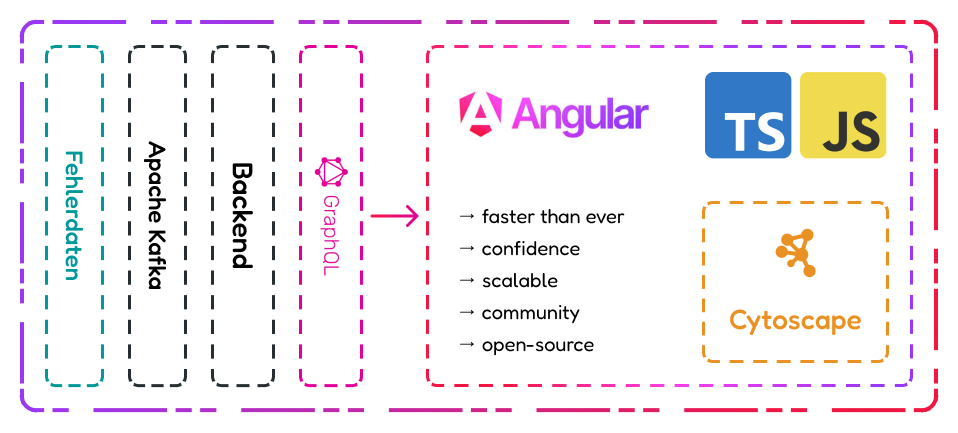
\includegraphics[width=0.8\textwidth]{content/img/Architecture/Architecture_Angular.jpg}
    \caption{Architektur unseres Prototypen mit Fokus auf das Frontend, welches mit Angular implementiert ist}
    \label{fig:ArchitectureFrontendAngular}
\end{figure}
\FloatBarrier

Google wirbt für das open-source Framework mit Schnelligkeit, Ausfallsicherheit aufgrund leichter Skalierbarkeit und einer unfassbar starken Community. Jedoch haben wir uns aus keinem dieser genannten Gründe für dieses Framework entschieden. Siemens hat uns wärmstens empfohlen, dass wir Angular verwenden sollen, wie Sie auch im Plichtenheft im Anhang sehen können. Das liegt daran, dass Siemens in Zukunft die Implementierung der Webapplikation wahrscheinlich, jedoch noch nicht zu 100\%, mit Angular durchführen will. Unsere Applikation wäre somit eine der ersten, welche das \emph{Corporate Design} von Siemens in einer echten Angular-Anwendung umsetzt. \cite{AngularFeatures}

Eines der bemerkenswertesten Features bei Angular ist die direkte Unterstützung der CLI (\emph{Command Line Interface}), sodass alle Aktionen mittels Terminal durchgeführt werden können. Diese Aktionen umfassen das Erstellen eines Projekts, das Hinzufügen von Bibliotheken, das Erstellen eines Komponenten bis hin zum Starten der Applikation. Summa summarum ist die CLI von Angular ein sehr umfangreiches, hilfreiches, mächtiges und von der Community geschätzes Tool, um das Angular Framework zu steuern und es hilft auch vor allem Programmierern, welche Angular neu erlernen, da die Einfachheit der Befehle nicht nur gut dokumentiert, sondern auch intuitiv sind. \cite{AngularCLI}

Beim Implementieren der Webapplikation habe ich die Angular CLI genutzt, um das Projekt und anschließend alle Komponenten zu erstellen. Zu den Komponenten kommt gleich noch mehr.

Außerdem hat Angular bereits einige moderne Features out of the box. Es unterstützt \emph{Server-Side Rendering}, ein Prozess, bei welchem bereits auf dem Server die gesamte HTML-Dateien gerendert werden und der Benutzer nicht auf extra JavaScript und CSS-Dateien warten muss, was die Ladezeiten deutlich verbessert. Angular ist zusätzlich kompatibel mit den beliebtesten CSS-Präprozessoren, wie zum Beispiel \wordindoublequotes{Sass}, \wordindoublequotes{less} und \wordindoublequotes{stylus}. Präprozessoren sind in diesem Sinn verbesserte und erweiterte Versionen des Grundgerüsts von CSS, welche das Schreiben dieser Beschreibungssprache mit unterschiedlichen Regeln erheblich erleichtern. Bevor der Browser diese Präprozessor-Daten anschließend jedoch interpretieren kann, müssen diese in reines CSS umgewandelt werden. Aus diesem Grund auch der Name \emph{Präprozessor}. \cite{AngularFeatures,AngularStyling}

Ich habe mich beim Erstellen des Projekts für die Verwendung von Sass entschieden, da ich in der Vergangenheit bei allen Projekten mit dieser erweiterten Version von CSS gearbeitet habe. Um genau zu sein, habe ich die \emph{SCSS}-Sytanx verwendet, da Sass zwei Syntaxen unterstützt, Sass und SCSS. Sass bietet einige Vorteile, darunter das Verschachteln von CSS-Blöcken, das Deklarieren von Variablen, Module, Mixins und vieles mehr. Allerdings habe ich das Server-Side Rendering deaktiviert. \cite{Sass}

Darüber hinaus hat Angular bereits ein eigenes Testsystem und Routing-System. Es kann mittels einfacher Installation des \mintinline{bash}{@angular/pwa} Pakets zu einer Progressive Web App gemacht werden und ist kompatibel mit unzähligen JavaScript-Bibliotheken auf dem Markt, wie zum Beispiel die ebenfalls von Google entwickelte UI-Bibliothek Angular Material, welche Standardkomponenten, wie zum Beispiel Slider, Toggle, Button, Datepicker usw. mit sich bringt. Die Möglichkeiten für Webapplikationen mit Angular sind heutzutage unbegrenzt. \cite{AngularTesting,AngularRouting,AngularMaterial}

In unserer Applikation wird das Testsystem nicht verwendet, weil keine Methoden zum Testen implementiert worden sind. Jedoch verfügt die Anwendung über die Funktionalität des Routings. Je nachdem, welche der drei Seiten Sie aufrufen -- Dashboard, Findings und Graph --, wird ein anderer Komponent gerendert. Die Verwendung der UI-Bibliothek Angular Material zieht sich bei der Applikation durch alle Seiten und Komponenten. \cite{AngularTesting,AngularRouting,AngularMaterial}

Angular basiert auf Komponenten. Dies sind kleinere, spezifische Teile des Frontends, welche innerhalb von anderen Komponenten oder unter gewissen Routen angezeigt werden können. Der Vorteil von Komponenten ist die Wiederverwendung des Codes, da jeder Komponent beliebig oft angezeigt werden kann. Jeder Komponent hat eine eigene Verwaltung der für diesen Komponenten relevanten Logik, ein eigenes CSS-Styling und HTML natürlich. Dadurch wird automatisch eine Art Entkoppelung der Logik im Frontend gewonnen. In einem \wordindoublequotes{Tic-Tac-Toe}-Spiel könnten Sie zum Beispiel einen Komponenten für ein einzelnes Kästchen programmieren, welcher die Logik für das Klicken dieses Feldes implementiert. \cite{AngularRouting,AngularComponents}

Wie bereits erwähnt, hat unsere Applikation einige Komponenten. Hierbei existiert eine Komponente, welche immer angezeigt wird, das ist die Navigation. Die drei anderen Hauptkomponenten (Dashboard, Findings und Graph) werden dynamisch, je nach URL angezeigt. Die letzte, selbst programmierte Angular Komponente in unserem System ist das Donatdiagramm, welches in eine eigene Komponente ausgelagert worden ist, damit es wiederverwendet werden kann.

In unserem Fall wird Angular nun verwendet, um die Daten des Stromnetzwerkes veranschaulich darzustellen. Dazu nutzt das Frontend die GraphQL-Schnittstelle, um geschickt an die Daten zu kommen. Beispielsweise wird nur eine einzige Query durchgeführt, um alle Daten in der Tabelle in Abbilung \ref{fig:PrototypTabelle} zu bekommen. Wundern Sie sich nicht: Die Daten sind anonymisiert.

\begin{figure}
    \centering
    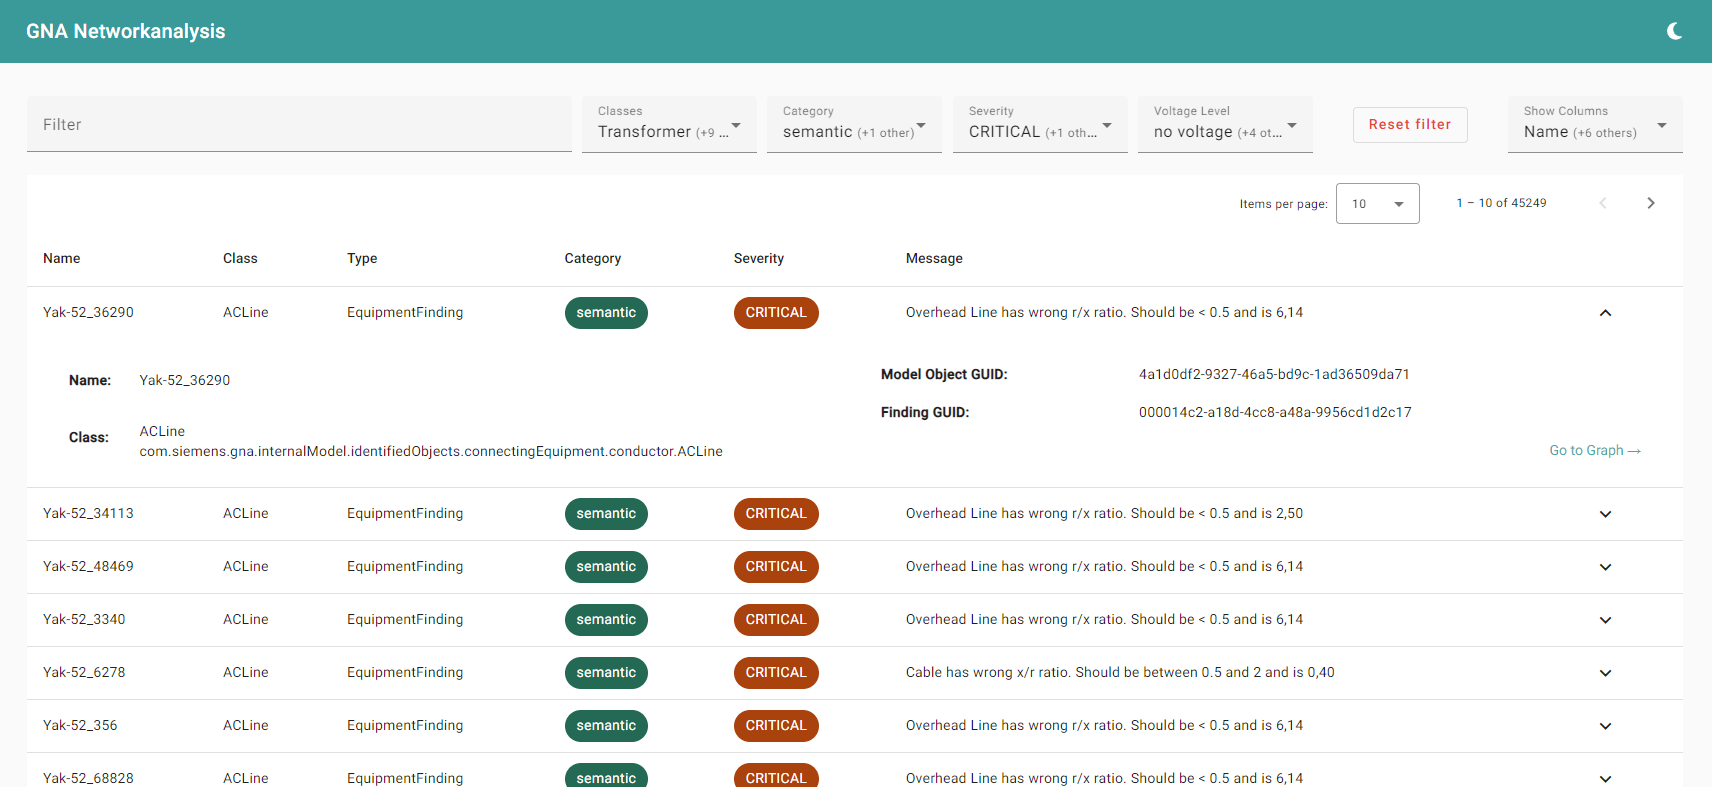
\includegraphics[width=1\textwidth]{content/img/Empire/Frontend/Angular_Findings_Prototype.png}
    \caption{Abbildung der Tabelle der Fehlerdaten im Stromnetzwerk mit Sortier- und Filteroptionen unseres Prototypen}
    \label{fig:PrototypTabelle}
\end{figure}
\FloatBarrier

\newpage

\subsection{Bibliothek zum Erstellen des Graphes: Cytoscape}

Aufgrund der unendlichen Möglichkeiten und vielfältigen Unterstützung mit anderen Bibliotheken, zählt auch die Cytoscape-Bibliothek zu einem leicht zu integrierenden Tool zur Visualisierung von Graphen. Die Bibliothek bietet eine umfassende Dokumentation aller Funktionen. Das Grundkonzept der Bibliothek basiert auf einer Liste von Elementen, welche die Knoten und Kanten gesammelt umfasst. Diese Knoten und Kanten werden über die Bibliothek in einem konfigurierbaren Layout in einen Canvas im HTML angezeigt. Cytoscape unterstützt dabei bereits alle notwendigen Animations- und Interaktionsmöglichkeiten für Maus und Finger (bei Touchdisplays). \cite{Cytoscape}

Unser Prototyp implementiert einen Graphen, welche die Objekte des Stromnetzwerkes (Umspannwerk, Leiter, Schalter, Widerstände, Generatoren, Verbraucher, ...) als Knoten in Verbindung setzt. Um diesen Graphen initial zu erstellen, werden mittels GraphQL die gesamten Objekte mit der Information über dessen Verbindungen zu anderen Objekten geladen und anschließend zu Knoten und Kanten aufbereitet (Quellcode \ref{lst:AufbereitungKnotenKantenGraphQLCytoscape},) sodass Cytoscape diese im Graphen rendern kann.

\begin{lstlisting}[language={JavaScript},caption={Erstellen der Knoten und Kanten mittels Liste von Objekten von GraphQL},label={lst:AufbereitungKnotenKantenGraphQLCytoscape},captionpos=b]
getNodeEdges(input: ModelObjectInput): Observable<GraphElement[]> {
  return this.modelObjectService.getModelObjects(input).pipe(
    switchMap((data) => {
      var modelObjectResult: ModelObjectResult = data;

      var nodes: GraphElement[] = [];
      var edges: GraphElement[] = [];

      /* calculate nodes and edges logic */

      return of([...nodes, ...edges] as GraphElement[]);
    })
  );
}
\end{lstlisting}

Diese Liste von Graph-Elementen wird anschließend an die Cytoscape-Bibliothek übergeben. Somit verwaltet nun Cytoscape die Objekte und wie diese im HTML Canvas gerendert werden.

\begin{lstlisting}[language={JavaScript},caption={Laden der Knoten und Kanten in den Graphen mittels Cytoscape},label={lst:GraphElementeLadenCytoscape},captionpos=b]
this.graphService.getNodeEdges(/* input */).subscribe((data) => {
  this.nodesEdges = data as GraphElement[];

  this.cy = cytoscape({
    container: document.getElementById('cy'),
    elements: this.nodesEdges as GraphElement[],
    style: this.stylesheet as Stylesheet[],
    layout: colaLayout,
  });
});
\end{lstlisting}

Wie Sie im Quellcode \ref{lst:GraphElementeLadenCytoscape} außerdem sehen können, wird das \wordindoublequotes{cola}-Layout verwendet, um die Knoten effizient im Viewport der Webseite zu positionieren. \wordindoublequotes{Cola} ist hierbei eines der Layouts, welches physikalische Gesetze aus der Natur nutzt, um die Kräfte zwischen den einzelnen Knoten zu berechnen und um diese gleichmäßig im Canvas zu verteilen. Viele weitere in Cytoscape integrierten Layouts, wie zum Beispiel \wordindoublequotes{cise}, \wordindoublequotes{cose-bilkent}, \wordindoublequotes{fcose}, \wordindoublequotes{d3-force} und \wordindoublequotes{euler}, basieren ebenfalls auf dieser Eigenschaft, sogenannt \wordindoublequotes{force-directed}. Der Grund für die Auswahl des \wordindoublequotes{cola}-Layouts ist die Funktionalität der unendlichen Ausführung (die Berechnungen der wirkenden Kräfte untereinander werden niemals gestoppt), welche sicherstellt, dass sich der Graph immer lebendig anfühlt. Falls die Ausführung enden würde, sähe der Graph nach Ablauf der Berechnungen tot aus, da Knoten nicht mehr aufeinander reagieren würden.